
% \chapter{Introduction}
\chapter{Introducere}
\label{cap:Introducere}
 \section{Contextul lucrării}
Conform statisticilor Poliției Române \cite{politia_romana}  în anul 2017 în România au fost 8624 de accidente rutiere în care 1951 oameni și-au pierdut viața iar 8172 oameni au fost răniți grav. Iar dacă ne uităm pe statiscticile întregii lumi \cite{WHO}  vedem că cca. 1,3 milioane de oameni mor anual în accidente rutiere.\newline
Statisticile de accidente ne arată că iar în 94\% dintre toate accidentele are rol și eroarea umană, iar 76\% sunt cauzate numai de eroare umană.
 Fred Wegman și Letty Aarts  în \cite{SWOV} prezintă căîn accidentele rutiere cei mai vulnerabili sunt pietonii (în special copiii) și bicicliștii fiind neprotejați. Locul doi pe lista de top a vulnerabilității o țin conducătorii de motociclete, mopeduri, etc. pentru că ei sunt numai parțial protejati (\ref{fig:lethalities}).\newline
%table with vulnerabilities in age and transport modes categories
\begin{figure}[h!]
    	\centering
	\captionsetup{justification=centering,margin=2cm}
	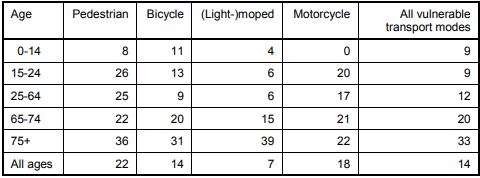
\includegraphics[width=0.9\textwidth]{figures/lethality_rates.png}
	\caption{Numărul de persoane implicate separate după vârstă și modul de transport pe 100 accidente serioase \cite{SWOV}}
	\label{fig:lethalities}
\end{figure}
Numerele acestea ridicate motivează aspirația noastră spre a construi sisteme inteligente care pot ne să ajute la evitarea acestor drame. Avem două asteptări cruciale față de un asemenea sistem: să funcționeze în timp real și să aibă o rată foarte ridicată de detecție corectă. Alarmele false sunt costisitoare și iritante pentru persoanele aflate în vehicul, iar greșelile în care sistemul nu recunoaște pericolul pot avea consecințe fatale.\newline
Pentru luarea deciziilor sistemul trebuie să obțină informațiile necesare din scenele de trafic, iar acest lucru se poate face prin mai multe modalități; în \cite{car_sensors}  Gert Rudolph și Uwe Voelzke prezintă cele mai folosite metode:
\begin{itemize}
	\item Camere video 360$^\circ$: fără îndoială imaginile video conțin peste 90\%de care are nevoie un conducător uman dar sunt potrivite și pentru conducerea vehiculelor autonome. Este critic ca camerele folosite să se descurce în toate condițiile de luminare.
	\item Radio Detection And Ranging (RADAR): sistemele ADAS (Advanced Driver Assistance Systems) necesită un număr de senzori, aceștia facând o contribuție la conducerea autonomăi. RADARele se folosesc în asistarea parcării, în recunoașterea situațiilor în care este nevoie de frânare imediată, măsurarea distanțelor, etc.
	\item Light Detection And Ranging (LiDAR): LiDAR este un sistem relativ nou în contextul vehiculelor autonome. LiDAR este un sistem bazat pe laser. Pe lângă \textit{transmitter} (laser) este nevoie și de un \textit{receiver} foarte sensibil. Folosit în primul rând pentru măsurarea distanțelor obiectelor staționare și a celor în mișcare, sistemul folosește proceduri speciale pentru construirea unei imagini 3D a obiectelor detectate.
	\item Sonare ultrasonice, GPS, senzori termale, etc.
\end{itemize}
Deși pentru oameni recunoașterea actorilor dintr-o scenă de trafic este o problemă trivială, pentru sistemele informatice este una dificilă, aceștia având nevoie de algoritmi isteți. Condițiile de luminare, vizibilitate precum și trăsăturile obiectelor (rotație, mărime, mișcare, culorile, etc.) sunt factori care îngreunează recunoașterea actorilor dintr-o scenă.
\section {Tema Lucrării}
Lucrarea de față se ocupă cu tema recunoașterii actorilor în imaginile captate din scene de trafic urban folosind inteligență artificială. Astfel se află la intersecția a două domenii care au primit foarte multă atenție recent: viziune artificială și inteligență artificială; cu algoritmi de procesare de imagini se vor extrage informații din imagini, iar cu ajutorul unei rețele neuronale se va face detectarea obiectelor în imaginile prelucreate precum și segmentarea semantică a imaginilor.\newline
De ce rețelele neuronale (convoluționale)? Putem să motivăm această decizie în următorul fel: să propunem că sarcina noastră este de a face un program care poate să recuoască un simplu cub, fără textură pe o imagine. Chiar și acest obiect simplu introduce mii de probleme: obiectul se poate roti, diferite condiții de luminare pot să încurce programul nostru. Și ce se întâmplă dacă cubul poate să aibă orice textură? Durere de cap! Am avea nevoie de pre-procesări ca să putem să tragem concluzii uniforme.\newline
Puterea rețelelor neuronale se află în faptul ca nu este nevoie de nicio trăsătură care diferențiază o categorie de obiecte de o altă categorie. Dacă rețeaua neuronală are un set de antrenare destul de mare, poate să tragă concluzii el însuși și să facă generalizări.

În viitorul apropiat o să avem nevoie de segmentare, pt că calculatoarele tre folosite, etc
Segmentarea imaginilor o chestie foarte bună: înțelegere, context, descompunere

In viata noastra de zi cu zi apar camere=> ar fi util sa intelegem ceea ce captureaza cu calculatoare

viziune artificiala + inteligenta artificiala
Ce se scrie aici:
\begin{itemize}
    \item Contextul
    \item Conturarea/Descrierea domeniului exact al temei
    \item Se răspunde la întrebările: \textbf{ce} (s-a făcut)?, \textbf{de ce} (s-a făcut, adică motivația; ce se rezolvă, la ce este util, etc.)?, \textbf{cum} (s-a făcut, adică particularitățile abordării, prezentate sumar).
    \item Introducerea se termină cu o descriere a conținutului lucrării, de genul: Cap X descrie ..., Cap Y prezintă ...
    \item Introducerea reprezintă o sinteză a lucrării, din care cititorul trebuie să-și poată da bine seama dacă lucrarea prezintă sau nu interes pentru el. 
    \item Se poate organiza pe subsecțiuni, dacă se dorește, după exemplul de mai jos, dar nu e obligatoriu asta, având în vedere dimensiunea mică
    \item reprezintă cca 5\% din lucrare (nu mai mult de 2-4 pagini)
\end{itemize}

Despre contextul în care este abordată și se aplică tema lucrării.

% \section{Report's Structure}
\section{Structura lucrării}
Capitolul~\ref{cap:obiective-specificatii} prezintă obiectivele \dots. Capitolul~\ref{cap:studiu-bibliografic} descrie \dots. În capitolul~\ref{cap:fund-teoretice} sunt prezentate \dots.
